\documentclass{article}
\usepackage[utf8]{inputenc}
\usepackage[utf8]{inputenc}

\usepackage[top=2cm, bottom=3.5cm, left=2.5cm, right=2.5cm]{geometry}

\usepackage{enumitem}
\usepackage{booktabs}
\usepackage[T1]{fontenc}
\usepackage{float}

\usepackage{graphicx}
\usepackage{epstopdf}

%
% The following macro is used to generate the header.
% Arguments are
% Course, Semester+Year, Homework number, Due Date, Student
%
\newcommand{\homework}[5]{
   \thispagestyle{plain}
   \newpage
   \noindent
   \begin{center}
   \framebox{
      \vbox{\vspace{2mm}
    \hbox to 6.28in { {\bf #1 \hfill #2} }
       \vspace{6mm}
       \hbox to 6.28in { {\Large \hfill Homework \##3 - Due date: #4\hfill} }
       \vspace{4mm}
       \hbox to 6.28in { {\hfill Student: #5} }
      \vspace{2mm}}
   }
   \end{center}
}

% Style of Greek letters
\renewcommand{\phi}{\varphi}
\renewcommand{\epsilon}{\varepsilon}

\usepackage{titlesec}
\renewcommand{\thesection}{\Roman{section}}
\titleformat{\section}
  {\mdseries\scshape\Large}{\Large{\mdseries\scshape Part }\thesection\ -\ }{0pt}{}
\titleformat{\subsection}
  {\mdseries\scshape\large}{\large{\mdseries\scshape Problem }\thesubsection\ -\ }{0pt}{}
\newcommand{\problem}{\subsection}

%%%%%%%%%%%%%%%%%%%%%% Macros EPFL-MLO %%%%%%%%%%%%%%%%%%%%%%%
\usepackage{amssymb,amsmath,amsthm,dsfont}

% Indicator function
\usepackage{bbm}
\providecommand{\ind}[1]{\mathbbm{1}_{\{#1\}}}

\providecommand{\lin}[1]{\ensuremath{\left\langle #1 \right\rangle}}
\providecommand{\abs}[1]{\ensuremath{\left\lvert#1\right\rvert}}
\providecommand{\norm}[1]{\ensuremath{\left\lVert#1\right\rVert}}

\providecommand{\refLE}[1]{\ensuremath{\stackrel{(\ref{#1})}{\leq}}}
\providecommand{\refEQ}[1]{\ensuremath{\stackrel{(\ref{#1})}{=}}}
\providecommand{\refGE}[1]{\ensuremath{\stackrel{(\ref{#1})}{\geq}}}
\providecommand{\refID}[1]{\ensuremath{\stackrel{(\ref{#1})}{\equiv}}}

  % basic sets
  \providecommand{\R}{\mathbb{R}} % Reals
  \providecommand{\N}{\mathbb{N}} % Naturals
  
  % random variables
  \DeclareMathOperator{\E}{{\mathbb E}}
  %\providecommand{\E}[1]{{\mathbb E}\left.#1\right. }     %expectation
  \providecommand{\Eb}[1]{\ensuremath{\E \left[#1\right] }} %expectation, with brackets
  \providecommand{\EE}[2]{\E_{#1} \! #2 }      %expectation  
  \providecommand{\EEb}[2]{\ensuremath{\E_{#1}\!\! \left[#2\right] }} %expectation,  with brackets
  \providecommand{\prob}[1]{\ensuremath{{\rm Pr}\left[#1\right] } }
  \providecommand{\Prob}[2]{\ensuremath{{\rm Pr}_{#1}\left[#2\right] } }
  \providecommand{\P}[1]{\ensuremath{{\rm Pr}\left.#1\right. }}
  \providecommand{\Pb}[1]{\ensuremath{{\rm Pr}\left[#1\right] }}
  \providecommand{\PP}[2]{\ensuremath{{\rm Pr}_{#1}\left[#2\right] }}
  \providecommand{\PPb}[2]{\ensuremath{{\rm Pr}_{#1}\left[#2\right] }}
  
  \newcommand\independent{\protect\mathpalette{\protect\independenT}{\perp}}
  \def\independenT#1#2{\mathrel{\rlap{$#1#2$}\mkern2mu{#1#2}}}

  % operators
  \DeclareMathOperator*{\argmin}{arg\,min}
  \DeclareMathOperator*{\argmax}{arg\,max}
  \DeclareMathOperator*{\supp}{supp}
  \DeclareMathOperator*{\diag}{diag}
  \DeclareMathOperator*{\Tr}{Tr}
  
  % bold vectors
  \providecommand{\0}{\mathbf{0}}
  \providecommand{\1}{\mathbf{1}}
  \renewcommand{\aa}{\mathbf{a}}
  \providecommand{\bb}{\mathbf{b}}
  \providecommand{\cc}{\mathbf{c}}
  \providecommand{\dd}{\mathbf{d}}
  \providecommand{\ee}{\mathbf{e}}
  \providecommand{\ff}{\mathbf{f}}
  \let\ggg\gg
  \renewcommand{\gg}{\mathbf{g}}
  \providecommand{\gv}{\mathbf{g}}
  \providecommand{\hh}{\mathbf{h}}
  \providecommand{\ii}{\mathbf{i}}
  \providecommand{\jj}{\mathbf{j}}
  \providecommand{\kk}{\mathbf{k}}
  \let\lll\ll
  \renewcommand{\ll}{\mathbf{l}}
  \providecommand{\mm}{\mathbf{m}}
  \providecommand{\nn}{\mathbf{n}}
  \providecommand{\oo}{\mathbf{o}}
  \providecommand{\pp}{\mathbf{p}}
  \providecommand{\qq}{\mathbf{q}}
  \providecommand{\rr}{\mathbf{r}}
  \renewcommand{\ss}{\mathbf{s}}
  \providecommand{\tt}{\mathbf{t}}
  \providecommand{\uu}{\mathbf{u}}
  \providecommand{\vv}{\mathbf{v}}
  \providecommand{\ww}{\mathbf{w}}
  \providecommand{\xx}{\mathbf{x}}
  \providecommand{\yy}{\mathbf{y}}
  \providecommand{\zz}{\mathbf{z}}
  
  % bold matrices
  \providecommand{\mA}{\mathbf{A}}
  \providecommand{\mB}{\mathbf{B}}
  \providecommand{\mC}{\mathbf{C}}
  \providecommand{\mD}{\mathbf{D}}
  \providecommand{\mE}{\mathbf{E}}
  \providecommand{\mF}{\mathbf{F}}
  \providecommand{\mG}{\mathbf{G}}
  \providecommand{\mH}{\mathbf{H}}
  \providecommand{\mI}{\mathbf{I}}
  \providecommand{\mJ}{\mathbf{J}}
  \providecommand{\mK}{\mathbf{K}}
  \providecommand{\mL}{\mathbf{L}}
  \providecommand{\mM}{\mathbf{M}}
  \providecommand{\mN}{\mathbf{N}}
  \providecommand{\mO}{\mathbf{O}}
  \providecommand{\mP}{\mathbf{P}}
  \providecommand{\mQ}{\mathbf{Q}}
  \providecommand{\mR}{\mathbf{R}}
  \providecommand{\mS}{\mathbf{S}}
  \providecommand{\mT}{\mathbf{T}}
  \providecommand{\mU}{\mathbf{U}}
  \providecommand{\mV}{\mathbf{V}}
  \providecommand{\mW}{\mathbf{W}}
  \providecommand{\mX}{\mathbf{X}}
  \providecommand{\mY}{\mathbf{Y}}
  \providecommand{\mZ}{\mathbf{Z}}
  \providecommand{\mLambda}{\mathbf{\Lambda}}
  
  % caligraphic
  \providecommand{\cA}{\mathcal{A}}
  \providecommand{\cB}{\mathcal{B}}
  \providecommand{\cC}{\mathcal{C}}
  \providecommand{\cD}{\mathcal{D}}
  \providecommand{\cE}{\mathcal{E}}
  \providecommand{\cF}{\mathcal{F}}
  \providecommand{\cG}{\mathcal{G}}
  \providecommand{\cH}{\mathcal{H}}
  \providecommand{\cI}{\mathcal{I}}
  \providecommand{\cJ}{\mathcal{J}}
  \providecommand{\cK}{\mathcal{K}}
  \providecommand{\cL}{\mathcal{L}}
  \providecommand{\cM}{\mathcal{M}}
  \providecommand{\cN}{\mathcal{N}}
  \providecommand{\cO}{\mathcal{O}}
  \providecommand{\cP}{\mathcal{P}}
  \providecommand{\cQ}{\mathcal{Q}}
  \providecommand{\cR}{\mathcal{R}}
  \providecommand{\cS}{\mathcal{S}}
  \providecommand{\cT}{\mathcal{T}}
  \providecommand{\cU}{\mathcal{U}}
  \providecommand{\cV}{\mathcal{V}}
  \providecommand{\cX}{\mathcal{X}}
  \providecommand{\cY}{\mathcal{Y}}
  \providecommand{\cW}{\mathcal{W}}
  \providecommand{\cZ}{\mathcal{Z}}

% Commenting
\RequirePackage[colorinlistoftodos,bordercolor=orange,backgroundcolor=orange!20,linecolor=orange,textsize=scriptsize]{todonotes}
\providecommand{\comment}[2]{\todo[inline,caption={}]{\textbf{#1: }#2}}%
\providecommand{\inlinecomment}[3]{%
  %\@getnewcolor%
  %\edef\@tempa{\@colstring}%
  {\color{#1}#2: #3}}%
\newcommand\commenter[2]%
{%
  \expandafter\newcommand\csname i#1\endcsname[1]{\inlinecomment{#2}{#1}{##1}}
  \expandafter\newcommand\csname #1\endcsname[1]{\comment{#1}{##1}}
}

% Use these for theorems, lemmas, proofs, etc.
\newtheorem{proposition}{Proposition}
\newtheorem{lemma}{Lemma}
\newtheorem{corollary}[lemma]{Corollary}
%\newtheorem{conjecture}[lemma]{Conjecture}
\newtheorem{definition}{Definition}
\newtheorem{remark}[lemma]{Remark}
\newtheorem{assumption}{Assumption}
\newtheorem{theorem}[lemma]{Theorem}
\newtheorem{example}[lemma]{Example}

\newtheorem{claim}{Claim}
\newtheorem{fact}{Fact}

\newcommand{\propositionautorefname}{Proposition}
\newcommand{\lemmaautorefname}{Lemma}
\newcommand{\corollaryautorefname}{Corollary}
\newcommand{\definitionautorefname}{Definition}
\newcommand{\remarkautorefname}{Remark}
\newcommand{\assumptionautorefname}{Assumption}
\newcommand{\theoremautorefname}{Theorem}
\newcommand{\exampleautorefname}{Example}
\newcommand{\claimautorefname}{Claim}
\newcommand{\factautorefname}{Fact}

\definecolor{mydarkblue}{rgb}{0,0.08,0.45}
\usepackage[colorlinks=true,linkcolor=blue]{hyperref} 
\hypersetup{ %
    colorlinks=true,
    linkcolor=mydarkblue,
    citecolor=mydarkblue,
    filecolor=mydarkblue,
    urlcolor=mydarkblue
}
\usepackage[capitalize,noabbrev]{cleveref}


\usepackage{url}
\def\UrlBreaks{\do\/\do-}

\usepackage[round]{natbib}
\renewcommand{\cite}[1]{\citep{#1}}



\begin{document}

\homework{Mathematics of Data}{Fall 2019}{4}{5\textsuperscript{th} January 2020}{Oriol Barbany Mayor}

\section{Projection-free convex low-rank matrix optimization}
\problem{Projection onto the nuclear norm ball}
\begin{enumerate}[label=(\alph*)]
    \item The projection of $Z$ onto $\cX$ is given by
    \begin{align}
        \Pi_{\cX}(Z)=\argmin_{X\in \cX}\norm{X-Z}_F
        \label{eq:prob}
    \end{align}
    
    Using Mirsky's inequality and the definition of Frobenius norm, it follows that
    \begin{align}
        \norm{X-Z}_F &\geq \norm{\Sigma_X - \Sigma_Z}_F := \sqrt{\sum_{i=1}^s\sum_{j=1}^s |\Sigma_X(i,j) - \Sigma_Z(i,j)|^2}\\
        &=\sqrt{\sum_{i=1}^s|\sigma_X(i) - \sigma_Z(i)|^2}=:\norm{\sigma_X - \sigma_Z}_2
    \end{align}
    where $\Sigma_X,\Sigma_Z\in \R^{s\times s}$ are the diagonal matrices of the singular values of $X,Z$ respectively.
    
    Using the latter, we have that
    \begin{align}
        \min_{X\in \cX}\norm{X-Z}_F \geq \min_{\Sigma_X\in \cX}\norm{\Sigma_X - \Sigma_Z}_F = \min_{\norm{\sigma_X}_1 \leq \kappa}\norm{\sigma_X - \sigma_Z}_2
        \label{eq:ineq}
    \end{align}
    so we can equivalently minimize the left hand side and obtain a solution for \eqref{eq:prob}. This latter has a minimum attained at $\sigma_X = \sigma_Z^{\ell_1}$, the projection of $\sigma_Z$ onto the $\ell_1-$norm ball of radius $\kappa$. This means that $\Sigma_Z^{\ell_1}:=\text{diag}(\sigma_Z^{\ell_1})$ minimizes the equivalent matrix version. Finally, using \eqref{eq:ineq} we have that
    \begin{align}
        \Pi_{\cX}(Z)=U\Sigma_Z^{\ell_1} V^T
    \end{align}
    
    \item After performing 10 runs, the projection took 1.452$\pm$0.129 and 77.376$\pm$3.188 seconds for the 1K and 1M MovieLens datasets respectively.
\end{enumerate}
\problem{LMO of nuclear norm}
\begin{enumerate}[label=(\alph*)]
    \item Let $Z=U\Sigma V^T$ be the singular value decomposition of $Z$ with $\sigma_{\max}$ its singular value and $\uu$ and $\vv$ the associated left and right singular vectors respectively. Since the matrices $U$ and $V$ are unitary,
    \begin{align}
         \lin{-\kappa \uu\vv^T, Z} &= Tr(-\kappa Z^T\uu\vv^T)= -\kappa Tr(V\Sigma U^T \uu\vv^T)= -\kappa \sigma_{\max} Tr(\vv \vv^T) = -\kappa  \sigma_{\max} Tr(\vv^T \vv) \\
         &= -\kappa \sigma_{\max} = -\kappa \norm{Z} \leq -\norm{X}_* \norm{Z} \leq -|\lin{X, Z}|\leq \lin{X, Z}
         \label{eq:lmo}
    \end{align}
    where the penultimate step holds by Hölder's inequality since the spectral norm is the dual of the nuclear norm. Given that $-\kappa \uu\vv^T \in \cX$, it follows that $-\kappa \uu\vv^T\in \text{lmo}_{\cX}(Z)$.
    
    \item After performing 10 runs, the projection took 0.029$\pm$0.005 and 0.294$\pm$0.008 seconds for the 1K and 1M MovieLens datasets respectively.
\end{enumerate}

\section{Crime Scene Investigation with Blind Deconvolution}
\begin{enumerate}[label=(\alph*)]
    \item
    \begin{lemma}
        For every linear operator $A:V\to W$, where $V$ and $W$ are finite-dimensional vector spaces, $A$ can be expressed as a matrix.
        \label{lemma:1}
    \end{lemma}
    \begin{proof}
        Let $\cB_V=\{\ee_1,\dots,\ee_n\}$ and $\cB_W=\{\ff_1,\dots,\ff_m\}$ be a basis of $V$ and $W$ respectively. By linearity of $A$, we know that
        \begin{align}
            A(c_1 \ee_1 + \cdots, c_n \ee_n) = c_1A(\ee_1) + \cdots + c_n A(\ee_n)
        \end{align}
        and thus the output of any vector $\xx \in V$ is fully determined by its decomposition in $\cB_V$ and $\{A(\ee_i)\}_{i=1}^n$. Moreover, since $A(\ee_i)\in W \ \forall i\in\{1,\dots,n\}$, it can be represented as a linear combination of basis vectors in $\cB_W$, i.e.
        \begin{align}
            T(\ee_i)=a_{i,1}\ff_1+\cdots+ a_{i,m}\ff_m
        \end{align}
        which means that the operator $A$ can be implemented as a $M\times N$ matrix.
    \end{proof}
    
    Using \autoref{lemma:1} and with a slight abuse of notation naming $A(X)=AX$ as the linear operator expressed as a matrix multiplication, we have that
    \begin{align}
        \nabla f(X) = A^T (AX - b)
    \end{align}
    
    Let $L$ be the Lipschitz constant of $\nabla f$.
    \begin{align}
        \norm{\nabla f(X) - \nabla f(X)} &= \norm{A^T (AX - b) - A^T (AY - b)}=\norm{A^TA(X - Y)} \\
        &\leq \norm{A^T A} \norm{X-Y} =: L \norm{X-Y}
    \end{align}
    where the inequality follows from the definition of the spectral norm.
    \item  The result with $\kappa=100$ and kernel support $K_1=K_2=17$ is depicted in \autoref{fig:deconv}, where one can easily read the plate with number J209LTL.
\end{enumerate}

\begin{figure}[ht]
    \centering
    \begin{minipage}{.45\textwidth}
        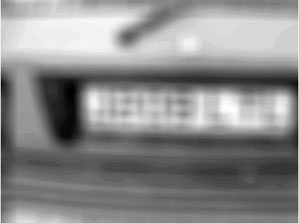
\includegraphics[width=\textwidth]{4-frank_wolfe/part2/blurredplate.jpg}
    \end{minipage}
    \begin{minipage}{.45\textwidth}
        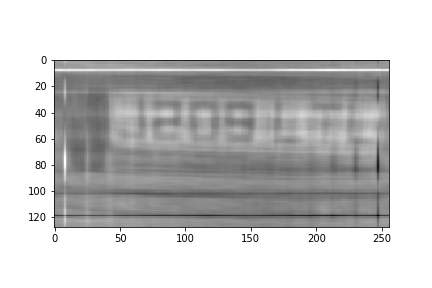
\includegraphics[width=\textwidth]{4-frank_wolfe/part2/reconstruction.jpg}
    \end{minipage}
    \caption{Blurred license plate (left) and result of the blind deconvolution (right).}
    \label{fig:deconv}
\end{figure}

\section{K-Means Clustering by Semidefinite Programming}
\problem{Conditional gradient method for clustering}
\begin{enumerate}[label=(\alph*)]
    \item
    Let $X, Y \in \cX$ any two matrices and $\alpha \in [0,1]$. Then, we have that $\alpha X + (1-\alpha)Y \in \cX$ and thus the set $\cX$ is convex iff $Tr(\alpha X + (1-\alpha)Y)\leq \kappa$ and $\alpha X + (1-\alpha)Y \succeq 0$.
    
    Given that the trace is a linear operator,
    \begin{align}
        Tr(\alpha X + (1-\alpha)Y) = \alpha Tr(X) + (1-\alpha)Tr(Y) \leq \alpha \kappa + (1-\alpha) \kappa = \kappa
    \end{align}
    where the inequality holds since $Tr(X),Tr(Y)\leq \kappa$.
    
    By definition of positive semidefiniteness,
    \begin{align}
        \alpha X + (1-\alpha)Y \succeq 0 \Longleftrightarrow \xx^T(\alpha X + (1-\alpha)Y) \xx \geq 0\qquad \forall \xx\in \R^p
    \end{align}
    
    Since $X,Y\succeq 0$,
    \begin{align}
        \xx^T(\alpha X + (1-\alpha)Y) \xx = \alpha \xx^T X \xx + (1-\alpha)\xx^T Y\xx  \geq 0
    \end{align}
    which concludes the proof.
    
    \item SDP relaxation can be formulated as
    \begin{align}
        \min_{X\in \cX} f(X) + g_1(A_1(X))+g_2(A_2(X)) \quad \text{ subject to }X\in \cK
    \end{align}
    where $g_1$ and $g_2$ are the indicator functions of singletons $\{b_1\}$ and $\{b_2\}$ respectively. Writing this constraints in the quadratic penalty form yields:
    \begin{align}
        g_1(A_1(X)) &\longrightarrow \text{QP}_{\{b_1\}}(X)=\min_{Y\in \{b_1\}}\norm{Y-A_1(X)}^2=\norm{b_1-A_1(X)}^2 \\
        g_2(A_2(X)) &\longrightarrow \text{QP}_{\{b_2\}}(X)=\min_{Y\in \{b_2\}}\norm{Y-A_2(X)}^2=\norm{b_2-A_2(X)}^2 \\
        X\in \cK &\longrightarrow \text{QP}_{\cK}(X)=\text{dist}^2(X,\cK)=\norm{\Pi_\cK(X) - X}^2
    \end{align}
    where $\Pi_\cK(X) = \argmin_{Y\in \cK}\norm{Y-X}$ is the projection of $X$ onto $\cK$.
    
    The penalized objective with penalization parameter $\frac{1}{2\beta}$ takes the form
    \begin{align}
        f(X)+\frac{1}{2\beta}\norm{b_1-A_1(X)}^2+\frac{1}{2\beta}\norm{b_2-A_2(X)}^2+\frac{1}{2\beta}\text{dist}^2(X,\cK)
    \end{align}
    which has a gradient of
    \begin{align}
        \nabla f(X) +\frac{1}{\beta}A_1^T(A_1X -b_1)+\frac{1}{\beta}A_2^T(A_2X-b_2)+\frac{1}{\beta}(X - \Pi_\cK(X))
        \label{eq:grad}
    \end{align}
    where I used \autoref{lemma:1} to express the linear operators $A_1,A_2$ as a matrix and Danskin's theorem to derivative as if $\Pi_\cK(X)$ was not a function of $X$.
    \item Following the proposed notation,
    \begin{align}
        v_k := \beta \nabla f(X_k) +A_1^T(A_1X_k -b_1)+A_2^T(A_2X_k-b_2)+(X_k - \Pi_\cK(X_k))
    \end{align}
    so the gradient found in \eqref{eq:grad} can be expressed as $\frac{v_k}{\beta}$.
    \item The initial k-means value is 150.9680, and after running the algorithm it drops to 28.7269. The final objective value is below the optimal value (51.63 and 57.05 respectively), which is due to the problem relaxation. This latter includes all the feasible solutions of the original problem and thus its optimal solution, but also includes others that are not feasible on the original problem.
\end{enumerate}

\end{document}